\section{Figures, Zitate, Mathe}
\begin{figure}[h]
\centering
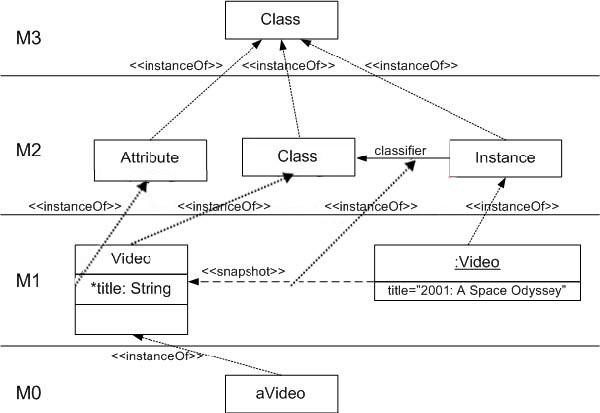
\includegraphics[scale=0.8]{OMG_MOF_4levels}
\caption{Das ist eine schlechte Grafik --- zu viele Pixel. Versuche Vektorgrafiken zu nutzen. Selbst malen geht gut mit draw.io powerpoint
  oder inkscape}\label{fig:mof}
\end{figure}

Wenn eine Abbildung verwendet wird, muss diese immer unbedingt im Text referenziert und beschrieben werden.
Z.B. so: \Cref{fig:mof}.

Zitieren geht so~\cite{haddadin2013towards}.

Math:

$A = \{x | x \in Y\}$

\begin{defs}\label{def:abc}
    A \textbf{Petrinet} is a tuple ${\Sigma = (P, T, F, W)}$.
\end{defs}

Petrinets are defined in~\Cref{def:abc}. See at the head of this document how to create your own definitions/lemma environments.

